\documentclass[a4paper,12pt]{article}
\usepackage{graphicx} 
\usepackage{hyperref}
\usepackage{float}
\usepackage{booktabs}
\usepackage{longtable}



% \begin{figure}[H]
%     \centering
%     \includegraphics[width=0.7\textwidth]{filename.png}
%     \caption{Your figure caption here.}
%     \label{fig:yourlabel}
% \end{figure}

\begin{document}

\title{Assignment 4 - Data Science\\
Disease Detection}
\author{Mohammad Hossein Basouli}
\date{\today}
\maketitle

\begin{center}
    \textit{\section*{Abstract}}
    \textit{In this analysis we try to apply multiple machine learning algorithms \& techniques to a dataset that contains symtoms related to eleven different diseases. 
    Some key findings of this analysis are: \textbf{Naive Bayes} performs really well when the features are binary - 
    \textbf{Ensembleing} of Different Methods usually increases the accuracy, by a few percentages - 
    Reduction of correlated features benefits accuracy of all of the algorithms (in this analysis).}
\end{center}

% ---------------------------------------------------------------------------------------------------------------------------------------------------------------------------------------------------------------------- %

\section{Introduction}

\subsection{Background:} Machine learning algorithms are commonly used at the intersection of Computer Science and Medicine to identify diseases based on specific symptoms. 
In this analysis, we will leverage these algorithms to classify 11 distinct diseases based on a given set of symptoms. 
The dataset, sourced from a Kaggle competition, includes a column labeled ID that identifies the case number, a label column specifying the disease associated with each case, 
and 64 features, numbered from 0 to 63. The dataset contains 564 rows and, as mentioned earlier, a total of 66 columns.  

\subsection{Objectives:} 
\begin{enumerate}
    \item Perform a basic \textit{Exploratory Data Analysis} step in order to understand the data.
    \item Start with selecting a handful of basic classfying algorithms such as \textit{Linear Discriminant Analysis}, \textit{SVM}, \textit{Naive Bayes}, etc. and find the best parameters for training those algorithms. 
    \item Evaluate your algorithms and see how well they are performing.
    \item Start exploring other methods such as \textit{Ensembling of The Previous Methods}, \textit{Bagging} and \textit{Boosting} methods.
    \item Try \textit{Feature Engineering} techniques such as \textit{Dimension Reduction}, etc.
    \item Examine the models to see what are the most important features.
\end{enumerate}

% ---------------------------------------------------------------------------------------------------------------------------------------------------------------------------------------------------------------------- %

\section{Exploratory Data Analysis}
\subsection{Correlation Matrix of the Features:}
\begin{figure}[H]
    \centering
    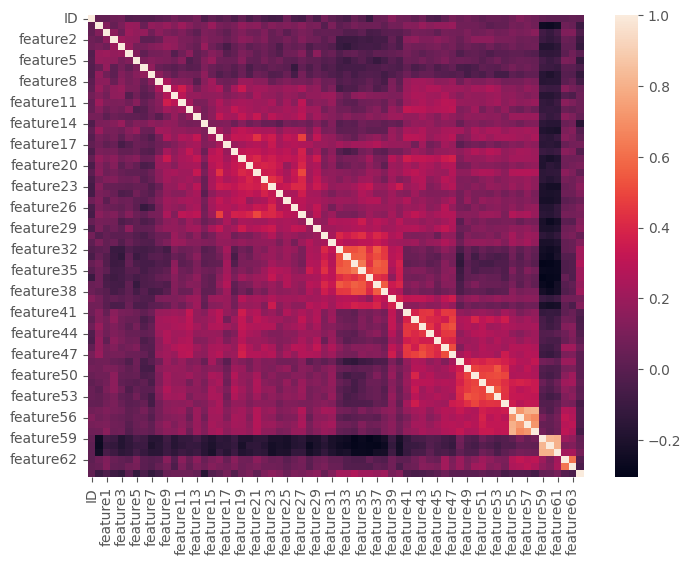
\includegraphics[width=0.7\textwidth]{./images/corr_mat.png}
    \caption{Correlation Matrix of the Features 0 through 63. The heatmap shows that the features \textit{feature56}, \textit{feature57} and \textit{feature58} are highly correlated. 
    This is also true for the features \textit{feature59}, \textit{feature60} and \textit{feature61}.}
    \label{fig:fig_1}
\end{figure}


\subsection{Proportion of the Data in Each Class:}
\begin{figure}[H]
    \centering
    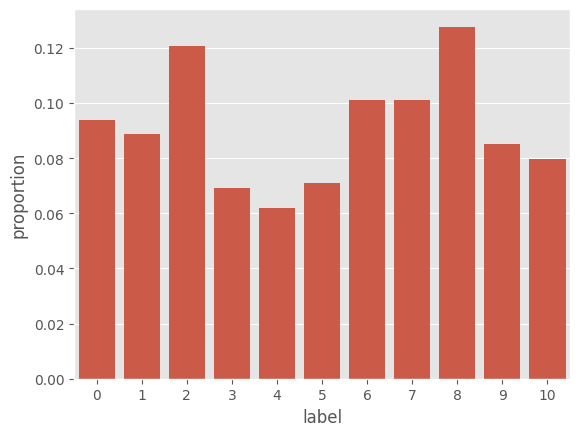
\includegraphics[width=0.7\textwidth]{./images/class_proror.png}
    \caption{Proportion of The Classes. This barplot shows that the data in the differet classes of the disease is approximately balance.}
    \label{fig:fig_2}
\end{figure}

% ---------------------------------------------------------------------------------------------------------------------------------------------------------------------------------------------------------------------- %

\section{Baseline Models}
We will summarize the results that we got with and without feature reduction (we have reduced the set of features to a smaller set, by replacing highly correlated features (Figure~\ref{fig:fig_1}) by a single one of them.) for each of the models separately.
We also can see that our algorithms perform slightly better after the feature reduction.

\subsection{Support Vector Machine}
\subsubsection{Hyperparameter Tuning:}
\begin{figure}[H]
    \centering
    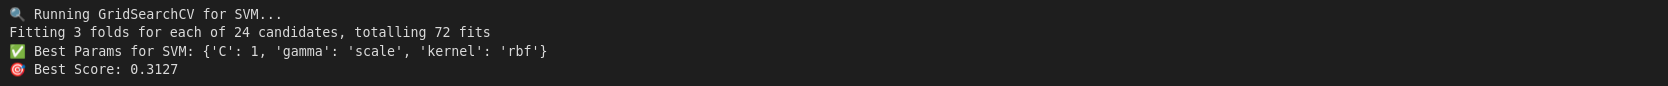
\includegraphics[width=0.7\textwidth]{./images/gssvm1.png}
    \caption{Grid Search Results for \textbf{SVM} Before Feature Reduction}
    \label{fig:fig_3}
\end{figure}
\begin{figure}[H]
    \centering
    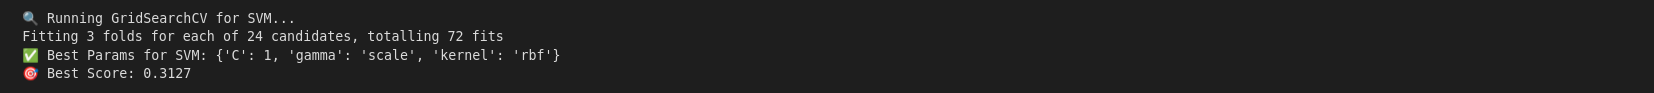
\includegraphics[width=0.7\textwidth]{./images/gssvm2.png}
    \caption{Grid Search Results for \textbf{SVM} After Feature Reduction}
    \label{fig:fig_4}
\end{figure}

\subsubsection{Evaluation:}
\begin{figure}[H]
    \centering
    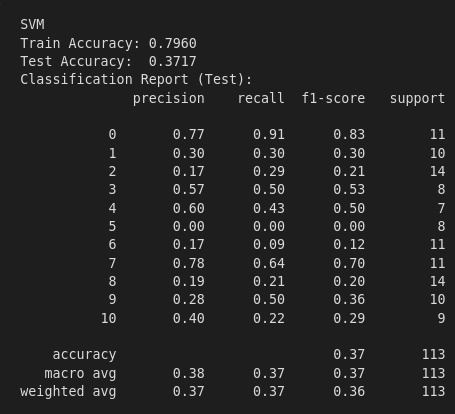
\includegraphics[width=0.7\textwidth]{./images/svmacc1.png}
    \caption{Accuracy Results for \textbf{SVM} Before Feature Reduction}
    \label{fig:fig_5}
\end{figure}
\begin{figure}[H]
    \centering
    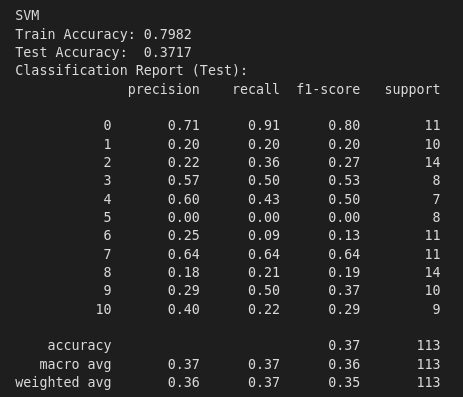
\includegraphics[width=0.7\textwidth]{./images/svmacc2.png}
    \caption{Accuracy Results for \textbf{SVM} After Feature Reduction}
    \label{fig:fig_6}
\end{figure}

\subsection{Logistic Regression}
\subsubsection{Hyperparameter Tuning:}
\begin{figure}[H]
    \centering
    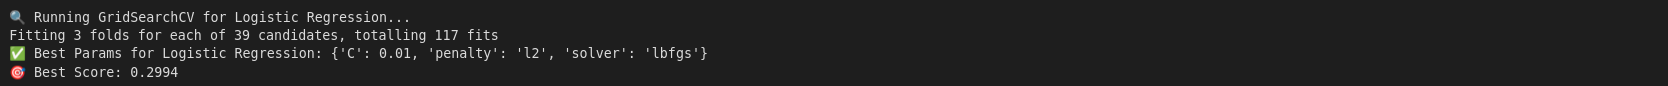
\includegraphics[width=0.7\textwidth]{./images/gslr1.png}
    \caption{Grid Search Results for \textbf{Logistic Regression} Before Feature Reduction}
    \label{fig:fig_7}
\end{figure}
\begin{figure}[H]
    \centering
    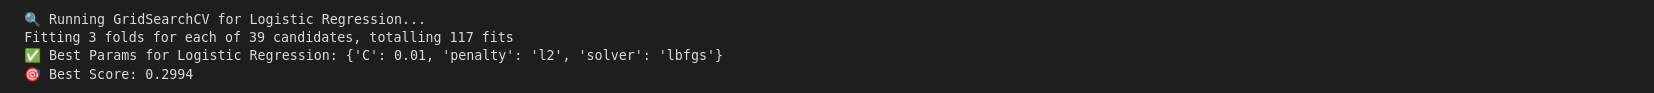
\includegraphics[width=0.7\textwidth]{./images/gslr2.png}
    \caption{Grid Search Results for \textbf{Logistic Regression} After Feature Reduction}
    \label{fig:fig_8}
\end{figure}

\subsubsection{Evaluation:}
\begin{figure}[H]
    \centering
    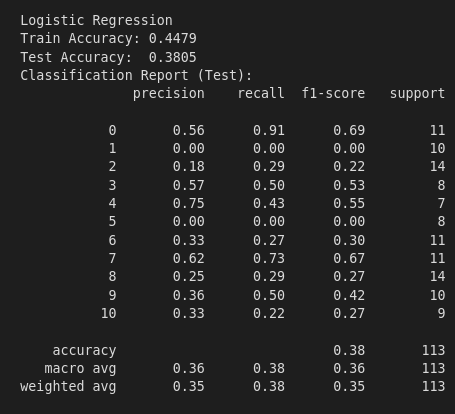
\includegraphics[width=0.7\textwidth]{./images/lracc1.png}
    \caption{Accuracy Results for \textbf{Logistic Regression} Before Feature Reduction}
    \label{fig:fig_9}
\end{figure}
\begin{figure}[H]
    \centering
    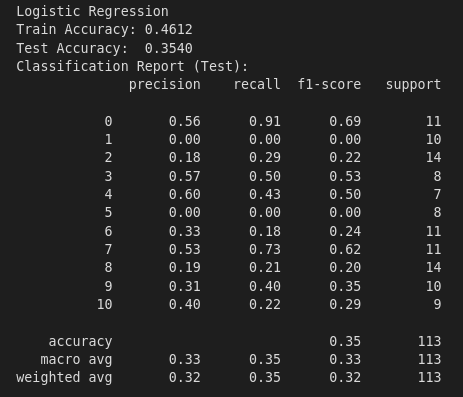
\includegraphics[width=0.7\textwidth]{./images/lracc2.png}
    \caption{Accuracy Results for \textbf{Logistic Regression} After Feature Reduction}
    \label{fig:fig_10}
\end{figure}

\subsection{Naive Bayes}
\subsubsection{Hyperparameter Tuning:}
\begin{figure}[H]
    \centering
    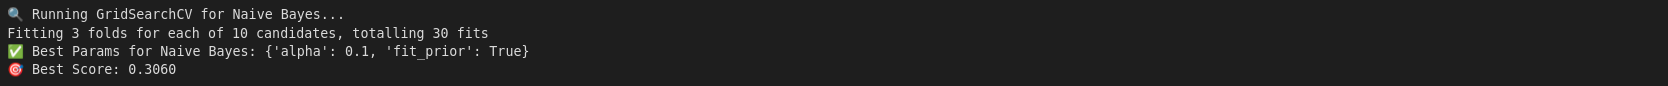
\includegraphics[width=0.7\textwidth]{./images/gsnb1.png}
    \caption{Grid Search Results for \textbf{Naive Bayes} Before Feature Reduction}
    \label{fig:fig_11}
\end{figure}
\begin{figure}[H]
    \centering
    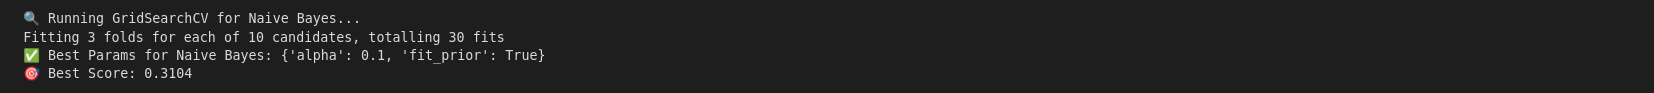
\includegraphics[width=0.7\textwidth]{./images/gsnb2.png}
    \caption{Grid Search Results for \textbf{Naive Bayes} After Feature Reduction}
    \label{fig:fig_12}
\end{figure}

\subsubsection{Evaluation:}
\begin{figure}[H]
    \centering
    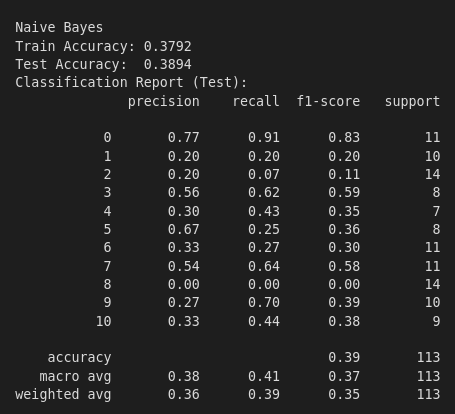
\includegraphics[width=0.7\textwidth]{./images/nbacc1.png}
    \caption{Accuracy Results for \textbf{Naive Bayes} Before Feature Reduction}
    \label{fig:fig_13}
\end{figure}
\begin{figure}[H]
    \centering
    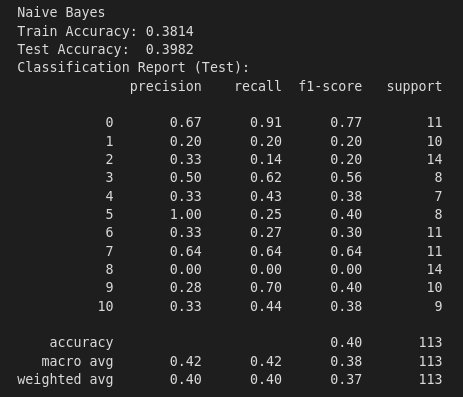
\includegraphics[width=0.7\textwidth]{./images/nbacc2.png}
    \caption{Accuracy Results for \textbf{Naive Bayes} After Feature Reduction}
    \label{fig:fig_14}
\end{figure}

\subsection{Linear Discriminant Analysis}
\subsubsection{Hyperparameter Tuning:}
\begin{figure}[H]
    \centering
    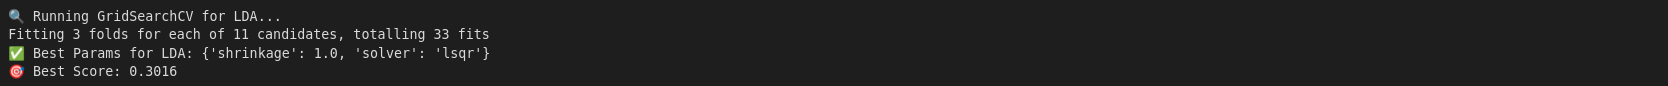
\includegraphics[width=0.7\textwidth]{./images/gslda1.png}
    \caption{Grid Search Results for \textbf{Linear Discriminant Analysis} Before Feature Reduction}
    \label{fig:fig_27}
\end{figure}
\begin{figure}[H]
    \centering
    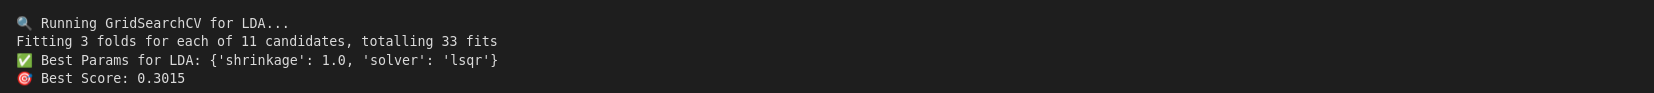
\includegraphics[width=0.7\textwidth]{./images/gslda2.png}
    \caption{Grid Search Results for \textbf{Linear Discriminant Analysis} After Feature Reduction}
    \label{fig:fig_28}
\end{figure}

\subsubsection{Evaluation:}
\begin{figure}[H]
    \centering
    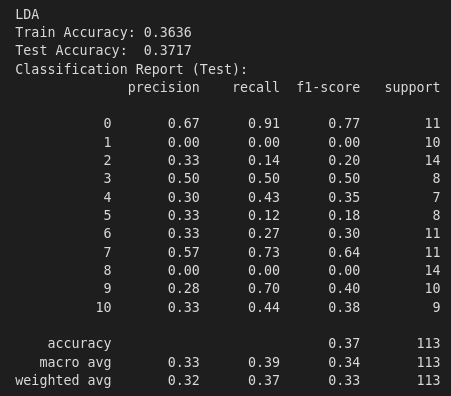
\includegraphics[width=0.7\textwidth]{./images/ldaacc1.png}
    \caption{Accuracy Results for \textbf{Linear Discriminant Analysis} Before Feature Reduction}
    \label{fig:fig_29}
\end{figure}
\begin{figure}[H]
    \centering
    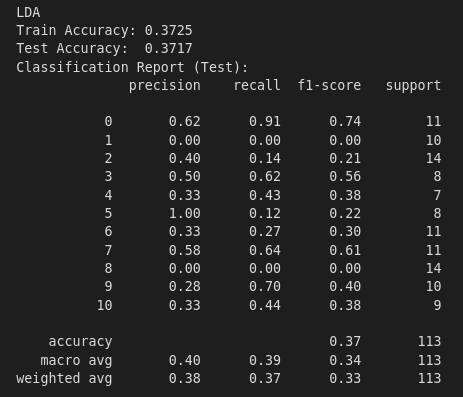
\includegraphics[width=0.7\textwidth]{./images/ldaacc2.png}
    \caption{Accuracy Results for \textbf{Linear Discriminant Analysis} After Feature Reduction}
    \label{fig:fig_30}
\end{figure}

% ---------------------------------------------------------------------------------------------------------------------------------------------------------------------------------------------------------------------- %

\section{Ensemble Models}
We will summarize the results that we got with and without feature reduction (we have reduced the set of features to a smaller set, by replacing highly correlated features (Figure~\ref{fig:fig_1}) by a single one of them.) for each of the ensemble models separately.
We can see that our algorithms perform slightly better after the feature reduction. We also observe that the performance of the ensembling methods is so much higher than the baseline models in general. 

\subsection{Random Forest}
\subsubsection{Hyperparameter Tuning:}
\begin{figure}[H]
    \centering
    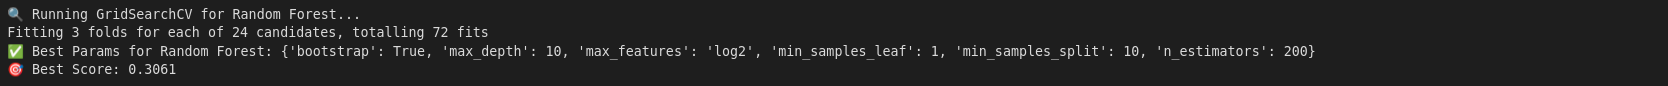
\includegraphics[width=0.7\textwidth]{./images/gsrf1.png}
    \caption{Grid Search Results for \textbf{Random Forest} Before Feature Reduction}
    \label{fig:fig_15}
\end{figure}
\begin{figure}[H]
    \centering
    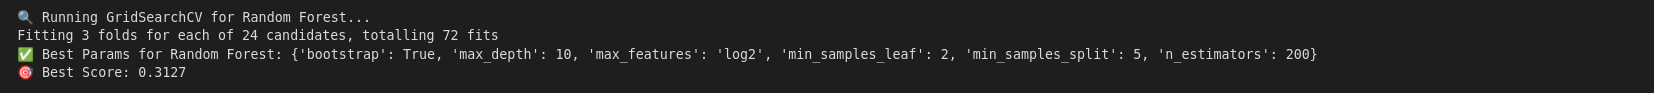
\includegraphics[width=0.7\textwidth]{./images/gsrf2.png}
    \caption{Grid Search Results for \textbf{Random Forest} After Feature Reduction}
    \label{fig:fig_16}
\end{figure}

\subsubsection{Evaluation:}
\begin{figure}[H]
    \centering
    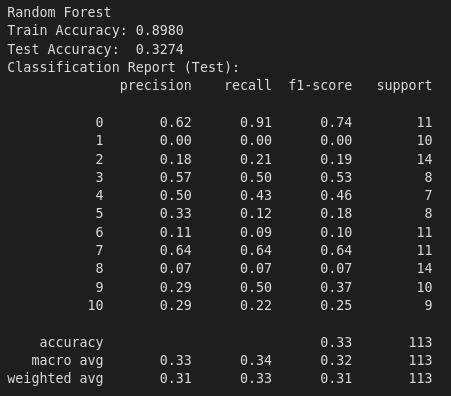
\includegraphics[width=0.7\textwidth]{./images/rfacc1.png}
    \caption{Accuracy Results for \textbf{Random Forest} Before Feature Reduction}
    \label{fig:fig_17}
\end{figure}
\begin{figure}[H]
    \centering
    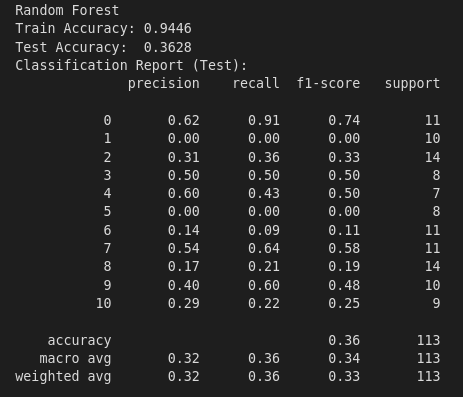
\includegraphics[width=0.7\textwidth]{./images/rfacc2.png}
    \caption{Accuracy Results for \textbf{Random Forest} After Feature Reduction}
    \label{fig:fig_18}
\end{figure}

\subsection{Ada Boost}
\subsubsection{Hyperparameter Tuning:}
\begin{figure}[H]
    \centering
    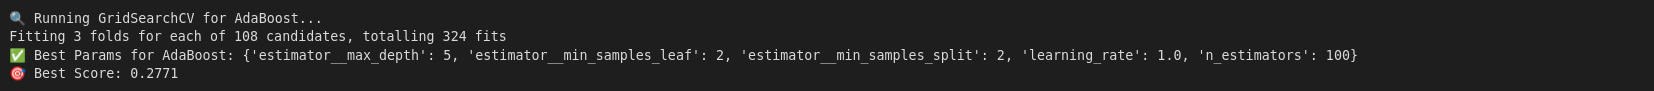
\includegraphics[width=0.7\textwidth]{./images/gsada1.png}
    \caption{Grid Search Results for \textbf{Ada Boost} Before Feature Reduction}
    \label{fig:fig_19}
\end{figure}
\begin{figure}[H]
    \centering
    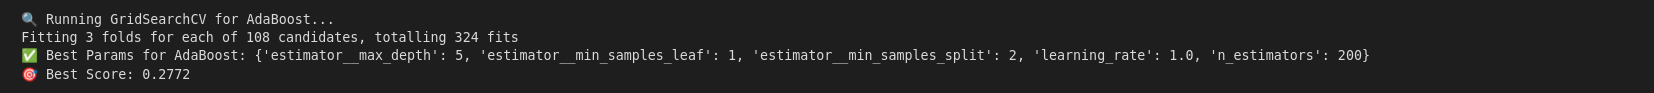
\includegraphics[width=0.7\textwidth]{./images/gsada2.png}
    \caption{Grid Search Results for \textbf{Ada Boost} After Feature Reduction}
    \label{fig:fig_20}
\end{figure}

\subsubsection{Evaluation:}
\begin{figure}[H]
    \centering
    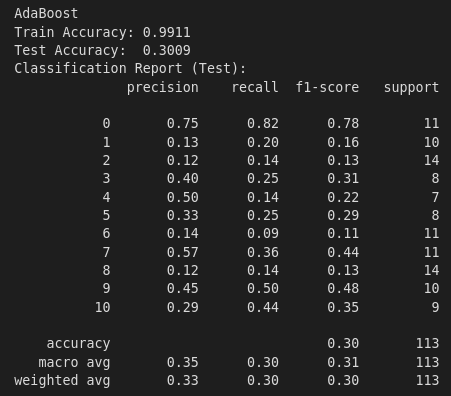
\includegraphics[width=0.7\textwidth]{./images/adaacc1.png}
    \caption{Accuracy Results for \textbf{Ada Boost} Before Feature Reduction}
    \label{fig:fig_21}
\end{figure}
\begin{figure}[H]
    \centering
    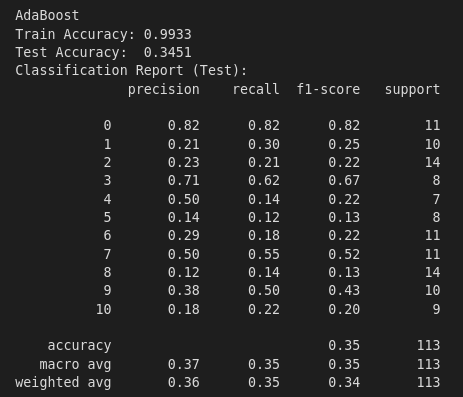
\includegraphics[width=0.7\textwidth]{./images/adaacc2.png}
    \caption{Accuracy Results for \textbf{Ada Boost} After Feature Reduction}
    \label{fig:fig_22}
\end{figure}

\subsection{XG Boost}
\subsubsection{Hyperparameter Tuning:}
\begin{figure}[H]
    \centering
    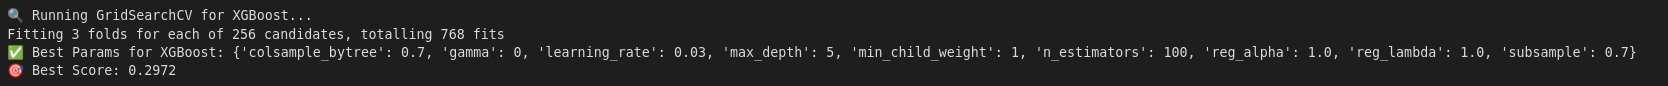
\includegraphics[width=0.7\textwidth]{./images/gsxgb1.png}
    \caption{Grid Search Results for \textbf{XG Boost} Before Feature Reduction}
    \label{fig:fig_23}
\end{figure}
\begin{figure}[H]
    \centering
    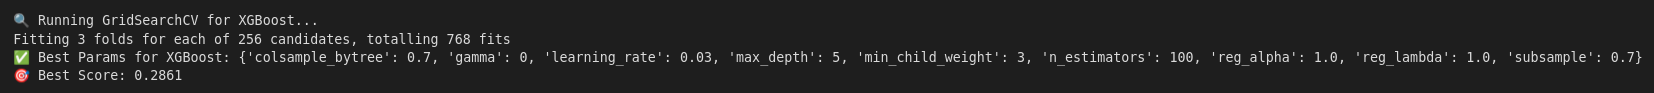
\includegraphics[width=0.7\textwidth]{./images/gsxg2.png}
    \caption{Grid Search Results for \textbf{XG Boost} After Feature Reduction}
    \label{fig:fig_24}
\end{figure}

\subsubsection{Evaluation:}
\begin{figure}[H]
    \centering
    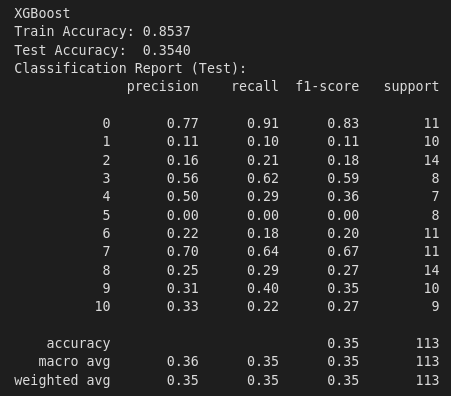
\includegraphics[width=0.7\textwidth]{./images/xgacc1.png}
    \caption{Accuracy Results for \textbf{XG Boost} Before Feature Reduction}
    \label{fig:fig_25}
\end{figure}
\begin{figure}[H]
    \centering
    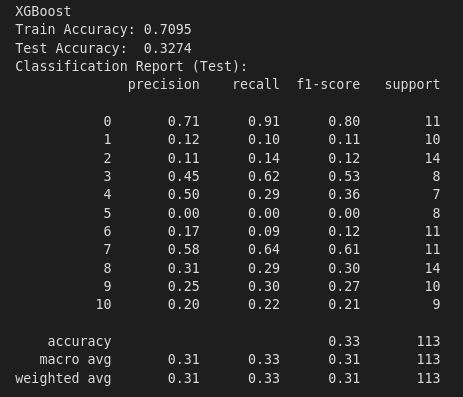
\includegraphics[width=0.7\textwidth]{./images/xgacc2.png}
    \caption{Accuracy Results for \textbf{XG Boost} After Feature Reduction}
    \label{fig:fig_26}
\end{figure}

\subsection{Voting Between All of The Models}
\subsubsection{Evaluation:}
\begin{figure}[H]
    \centering
    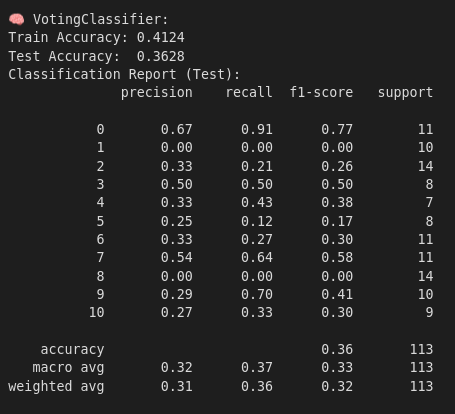
\includegraphics[width=0.7\textwidth]{./images/votacc1.png}
    \caption{Accuracy Results for \textbf{Voting Classifier} (Mix of all of the models) Before Feature Reduction}
    \label{fig:fig_31}
\end{figure}
\begin{figure}[H]
    \centering
    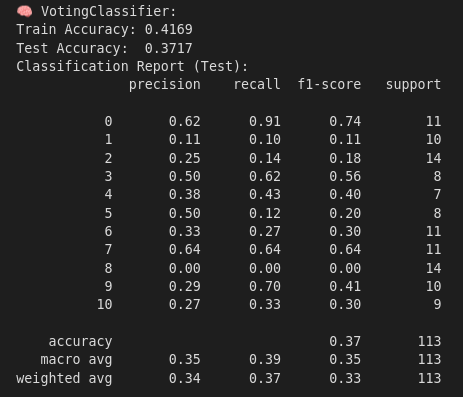
\includegraphics[width=0.7\textwidth]{./images/votacc2.png}
    \caption{Accuracy Results for \textbf{XG Boost} (Mix of all of the models) After Feature Reduction}
    \label{fig:fig_32}
\end{figure}

% ---------------------------------------------------------------------------------------------------------------------------------------------------------------------------------------------------------------------- %

\section{Feature Importance:}
\subsection{Feature Importance via MDI in Random Forest:}
\begin{figure}[H]
    \centering
    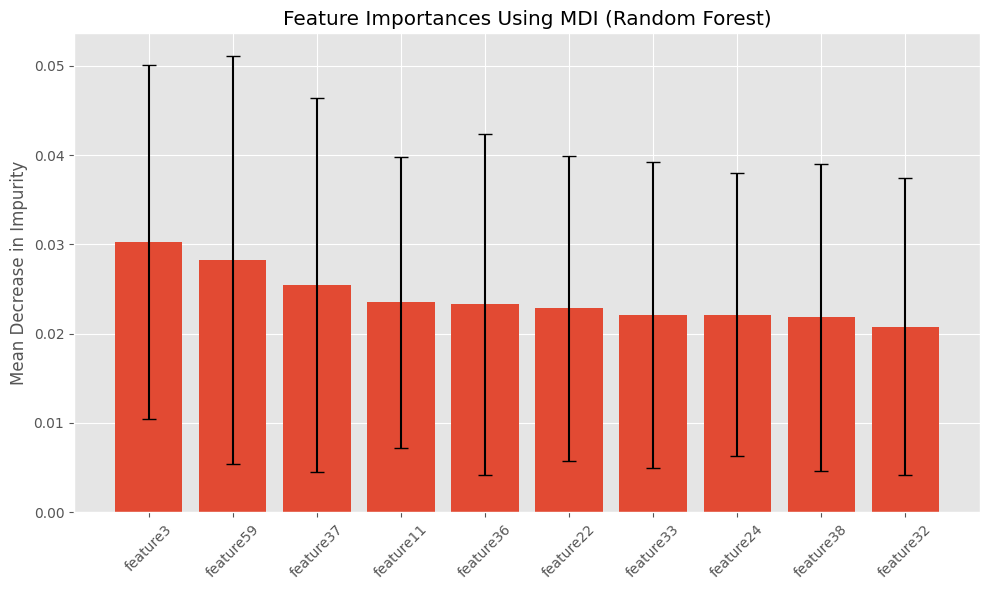
\includegraphics[width=0.7\textwidth]{./images/feature_impor_mdi.png}
    \caption{Feature Importance via MDI in \textbf{Random Forest}}
    \label{fig:fig_33}
\end{figure}

\subsection{Feature Importance via Permutation Test in Random Forest:}
\begin{figure}[H]
    \centering
    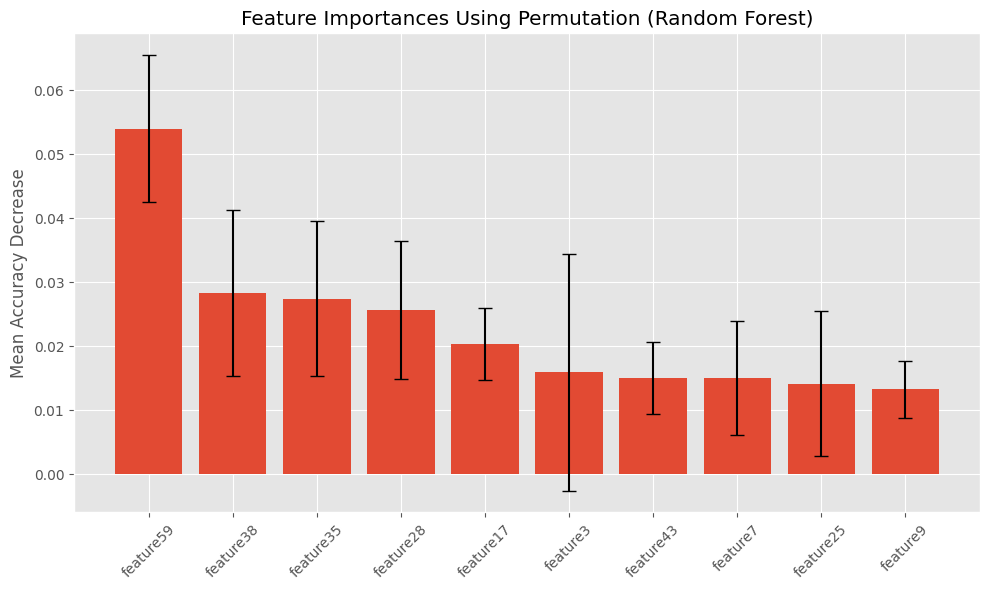
\includegraphics[width=0.7\textwidth]{./images/feature_impor_perm.png}
    \caption{Feature Importance via Permutation Test in \textbf{Random Forest}}
    \label{fig:fig_34}
\end{figure}

% ---------------------------------------------------------------------------------------------------------------------------------------------------------------------------------------------------------------------- %

\section{Conclusion:}
Our conclusion is that the \textbf{Ensembling Methods} such as \textbf{Random Forest}, \textbf{Voting}, etc outperform single, baseline methods like \textbf{Logistic Regression}, \textbf{LDA}, etc. in general. 
Also we saw that the feature reduction worked pretty well on this dataset and led to better results.   

\end{document}